\documentclass{article}
\usepackage{tikz}
\usetikzlibrary{arrows.meta, positioning, decorations.markings}

\begin{document}

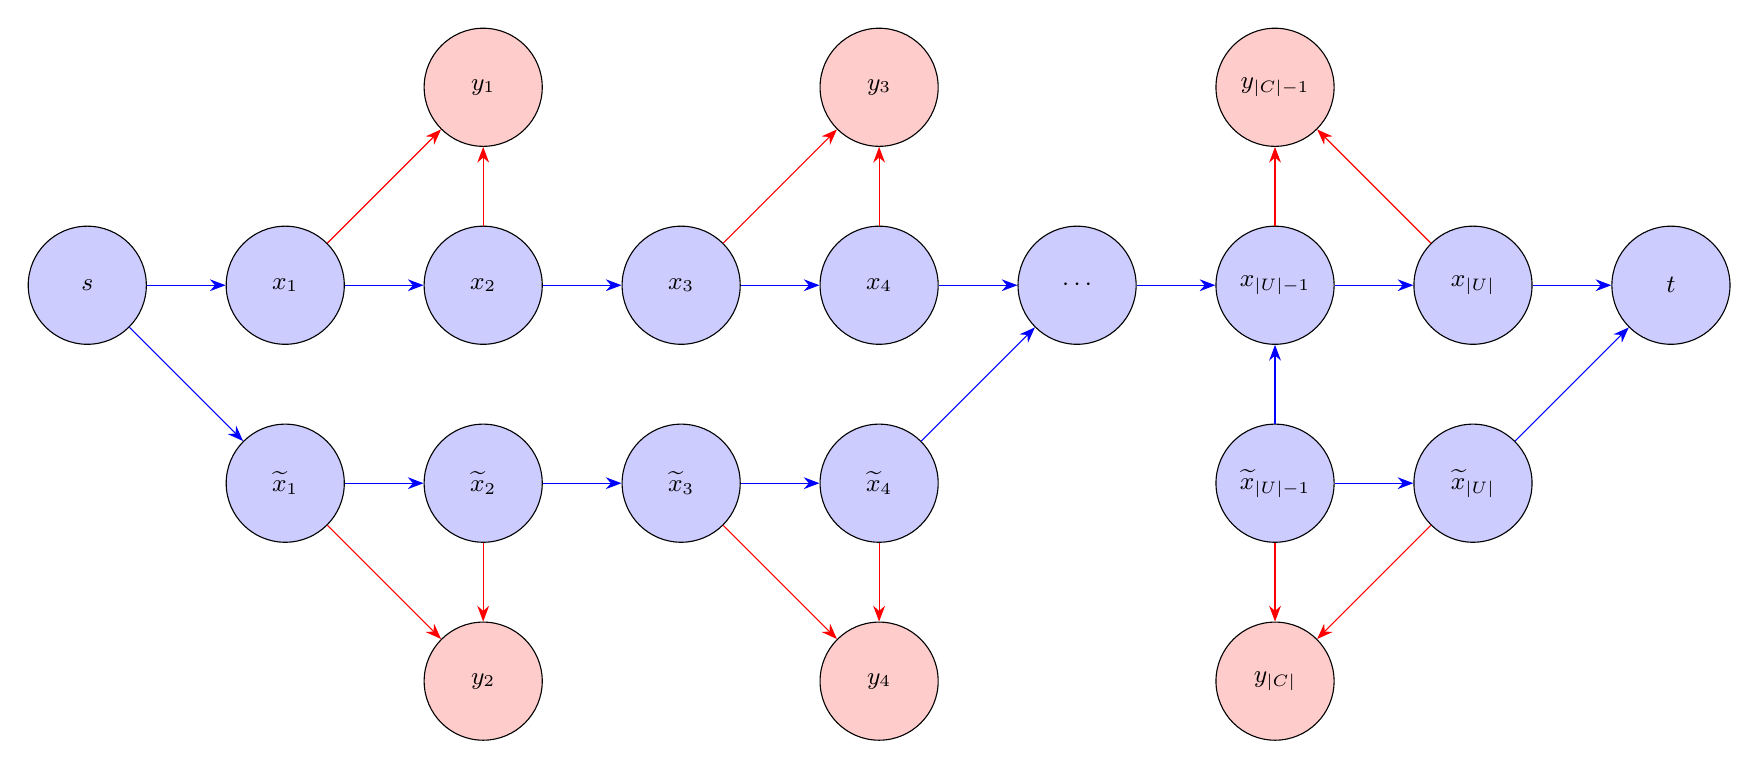
\begin{tikzpicture}[
    vertex/.style={circle, draw, minimum size=15mm},
    edge/.style={-{Stealth[length=2mm]}, blue},
    weighted edge/.style={-{Stealth[length=2mm]}, red},
    every node/.style={font=\small}
]
    % Draw vertices for the left part
    \node[vertex, fill=blue!20] (s) {\(s\)};
    \node[vertex, fill=blue!20, right=of s] (x1) {\(x_1\)};
    \node[vertex, fill=blue!20, right=of x1] (x2) {\(x_2\)};
    \node[vertex, fill=blue!20, right=of x2] (x3) {\(x_3\)};
    \node[vertex, fill=blue!20, right=of x3] (x4) {\(x_4\)};
    \node[vertex, fill=blue!20, right=of x4] (dots1) {\(\cdots\)};
    \node[vertex, fill=blue!20, right=of dots1] (xU1) {\(x_{|U|-1}\)};
    \node[vertex, fill=blue!20, right=of xU1] (xU) {\(x_{|U|}\)};
    \node[vertex, fill=blue!20, right=of xU] (t) {\(t\)};
    
    % Draw vertices for the left part (lower row)
    \node[vertex, fill=blue!20, below=of x1] (x~1) {\(\widetilde{x}_1\)};
    \node[vertex, fill=blue!20, below=of x2] (x~2) {\(\widetilde{x}_2\)};
    \node[vertex, fill=blue!20, below=of x3] (x~3) {\(\widetilde{x}_3\)};
    \node[vertex, fill=blue!20, below=of x4] (x~4) {\(\widetilde{x}_4\)};
    \node[vertex, fill=blue!20, below=of xU1] (x~U1) {\(\widetilde{x}_{|U|-1}\)};
    \node[vertex, fill=blue!20, below=of xU] (x~U) {\(\widetilde{x}_{|U|}\)};
    
    % Draw vertices for the additional parts (red)
    \node[vertex, fill=red!20, above=of x2] (y1) {\(y_1\)};
    \node[vertex, fill=red!20, above=of x4] (y3) {\(y_3\)};
    \node[vertex, fill=red!20, below=of x~2] (y2) {\(y_2\)};
    \node[vertex, fill=red!20, below=of x~4] (y4) {\(y_4\)};
    \node[vertex, fill=red!20, above=of xU1] (yC-1) {\(y_{|C|-1}\)};
    \node[vertex, fill=red!20, below=of x~U1] (yC) {\(y_{|C|}\)};
    
    % Draw edges for the left part (blue)
    \draw[edge] (s) -- (x1);
    \draw[edge] (s) -- (x~1);
    \draw[edge] (x1) -- (x2);
    \draw[edge] (x~1) -- (x~2);
    \draw[edge] (x2) -- (x3);
    \draw[edge] (x~2) -- (x~3);
    \draw[edge] (x3) -- (x4);
    \draw[edge] (x~3) -- (x~4);
    \draw[edge] (x4) -- (dots1);
    \draw[edge] (x~4) -- (dots1);
    \draw[edge] (dots1) -- (xU1);
    \draw[edge] (x~U1) -- (xU1);
    \draw[edge] (xU1) -- (xU);
    \draw[edge] (x~U1) -- (x~U);
    \draw[edge] (xU) -- (t);
    \draw[edge] (x~U) -- (t);
    
    % Draw weighted edges (red)
    \draw[weighted edge] (x1) -- (y1);
    \draw[weighted edge] (x2) -- (y1);
    \draw[weighted edge] (x3) -- (y3);
    \draw[weighted edge] (x4) -- (y3);
    \draw[weighted edge] (x~1) -- (y2);
    \draw[weighted edge] (x~2) -- (y2);
    \draw[weighted edge] (x~3) -- (y4);
    \draw[weighted edge] (x~4) -- (y4);
    \draw[weighted edge] (xU1) -- (yC-1);
    \draw[weighted edge] (x~U1) -- (yC);
    \draw[weighted edge] (xU) -- (yC-1);
    \draw[weighted edge] (x~U) -- (yC);
    
\end{tikzpicture}

\end{document}